\documentclass[letterpaper,12pt]{article}
\usepackage[margin=.65in,top=.72in,bottom=.62in,headheight=16pt,headsep=15pt,footskip=19pt]{geometry}
\usepackage[T1]{fontenc}
\usepackage{lmodern,tikz,fancyhdr}\pdfmapfile{+lm.map}
\usetikzlibrary{arrows.meta,shapes.geometric}
\pagestyle{fancy}\fancyhf{}\renewcommand{\headrulewidth}{0pt}\renewcommand{\footrulewidth}{0pt}
\setlength{\parindent}{0pt}\setlength{\parskip}{0pt}
\fancyhead[L]{\small Week 44 / The bag that copies / Grades 4--5}
\fancyfoot[L]{\footnotesize Bellingham Math Circle / Week 44 / W44-grades-4-5-v2}\fancyfoot[R]{\footnotesize\thepage}
\begin{document}
\noindent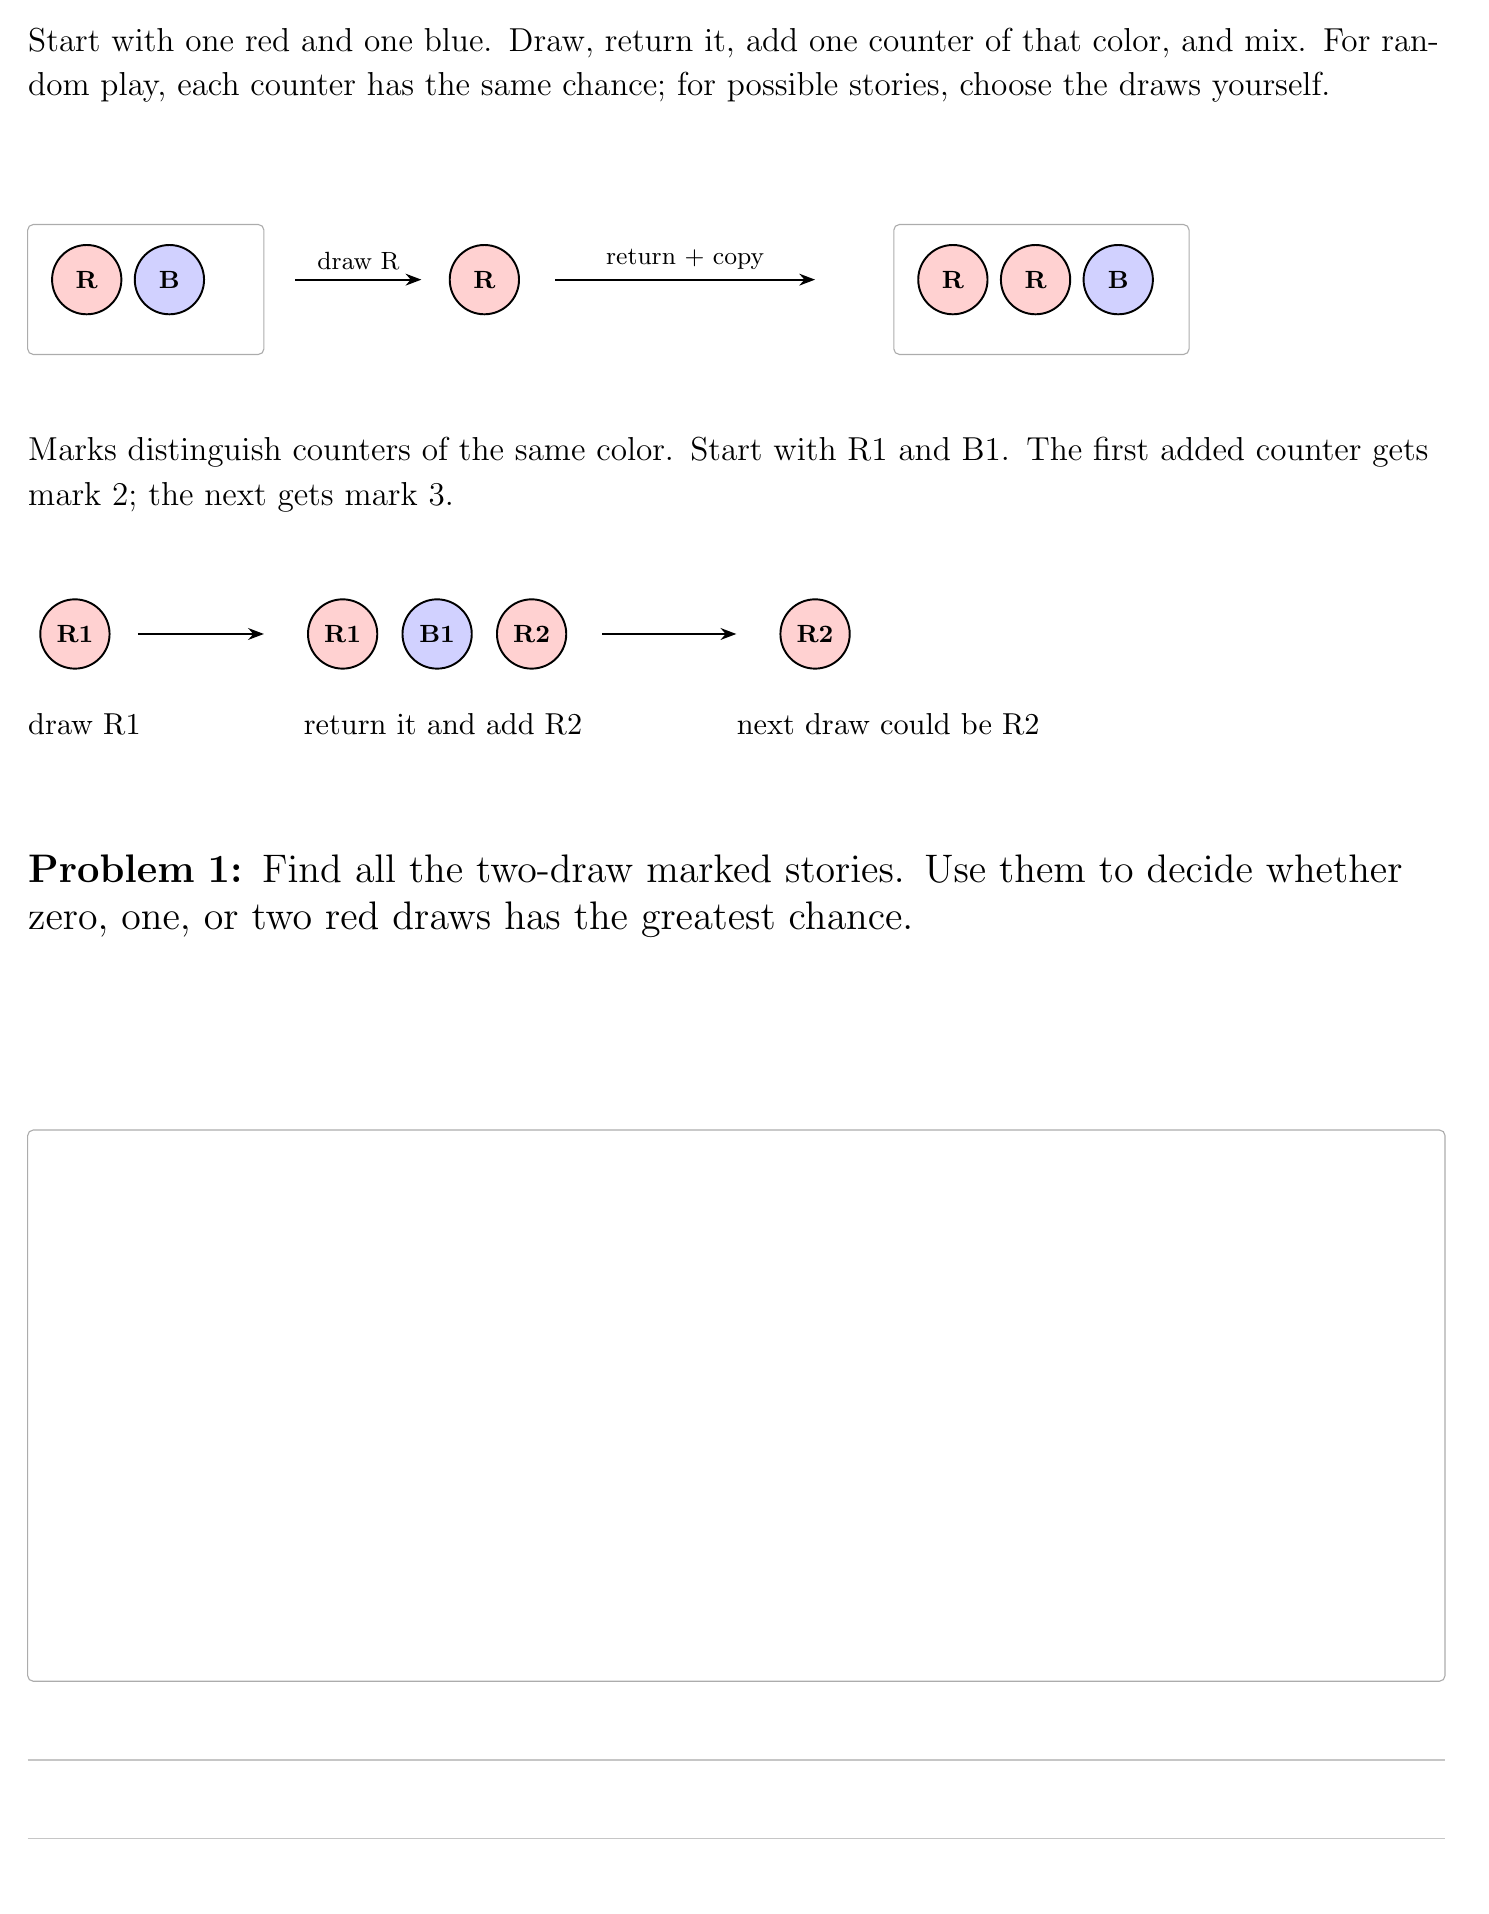
\begin{tikzpicture}[x=1cm,y=1cm]\path[use as bounding box] (0,0) rectangle (18.2,-23.6);
\node[anchor=north west,text width=18cm,inner sep=0pt,font=\fontsize{13}{16}\selectfont] at (0,0) {Start with one red and one blue. Draw, return it, add one counter of that color, and mix. For random play, each counter has the same chance; for possible stories, choose the draws yourself.};
\draw[gray!65,rounded corners=2pt] (0,-2.5) rectangle (3,-4.15);
\draw[fill=red!18,line width=.7pt] (0.75,-3.2) circle (0.44);
\node[font=\bfseries\small] at (0.75,-3.2) {R};
\draw[fill=blue!18,line width=.7pt] (1.8,-3.2) circle (0.44);
\node[font=\bfseries\small] at (1.8,-3.2) {B};
\draw[-{Stealth[length=2mm]},line width=.8pt] (3.4,-3.2) -- (5,-3.2) node[midway,above,font=\small] {draw R};
\draw[fill=red!18,line width=.7pt] (5.8,-3.2) circle (0.44);
\node[font=\bfseries\small] at (5.8,-3.2) {R};
\draw[-{Stealth[length=2mm]},line width=.8pt] (6.7,-3.2) -- (10,-3.2) node[midway,above,font=\small] {return + copy};
\draw[gray!65,rounded corners=2pt] (11,-2.5) rectangle (14.75,-4.15);
\draw[fill=red!18,line width=.7pt] (11.75,-3.2) circle (0.44);
\node[font=\bfseries\small] at (11.75,-3.2) {R};
\draw[fill=red!18,line width=.7pt] (12.8,-3.2) circle (0.44);
\node[font=\bfseries\small] at (12.8,-3.2) {R};
\draw[fill=blue!18,line width=.7pt] (13.85,-3.2) circle (0.44);
\node[font=\bfseries\small] at (13.85,-3.2) {B};
\node[anchor=north west,text width=18cm,inner sep=0pt,font=\fontsize{13}{16}\selectfont] at (0,-5.2) {Marks distinguish counters of the same color. Start with R1 and B1. The first added counter gets mark 2; the next gets mark 3.};
\draw[fill=red!18,line width=.7pt] (0.6,-7.7) circle (0.44);
\node[font=\bfseries\small] at (0.6,-7.7) {R1};
\draw[-{Stealth[length=2mm]},line width=.8pt] (1.4,-7.7) -- (3,-7.7) node[midway,above,font=\small] {};
\draw[fill=red!18,line width=.7pt] (4,-7.7) circle (0.44);
\node[font=\bfseries\small] at (4,-7.7) {R1};
\draw[fill=blue!18,line width=.7pt] (5.2,-7.7) circle (0.44);
\node[font=\bfseries\small] at (5.2,-7.7) {B1};
\draw[fill=red!18,line width=.7pt] (6.4,-7.7) circle (0.44);
\node[font=\bfseries\small] at (6.4,-7.7) {R2};
\draw[-{Stealth[length=2mm]},line width=.8pt] (7.3,-7.7) -- (9,-7.7) node[midway,above,font=\small] {};
\draw[fill=red!18,line width=.7pt] (10,-7.7) circle (0.44);
\node[font=\bfseries\small] at (10,-7.7) {R2};
\node[anchor=north west,text width=3cm,inner sep=0pt,font=\fontsize{11}{14}\selectfont] at (0,-8.7) {draw R1};
\node[anchor=north west,text width=5cm,inner sep=0pt,font=\fontsize{11}{14}\selectfont] at (3.5,-8.7) {return it and add R2};
\node[anchor=north west,text width=8cm,inner sep=0pt,font=\fontsize{11}{14}\selectfont] at (9,-8.7) {next draw could be R2};
\node[anchor=north west,text width=18cm,inner sep=0pt,font=\fontsize{14}{17}\selectfont] at (0,-10.5) {\textbf{Problem 1:} Find all the two-draw marked stories. Use them to decide whether zero, one, or two red draws has the greatest chance.};
\draw[gray!65,rounded corners=2pt] (0,-14) rectangle (18,-21);
\draw[gray!45] (0,-22) -- (18,-22);
\draw[gray!45] (0,-23) -- (18,-23);
\end{tikzpicture}
\newpage
\noindent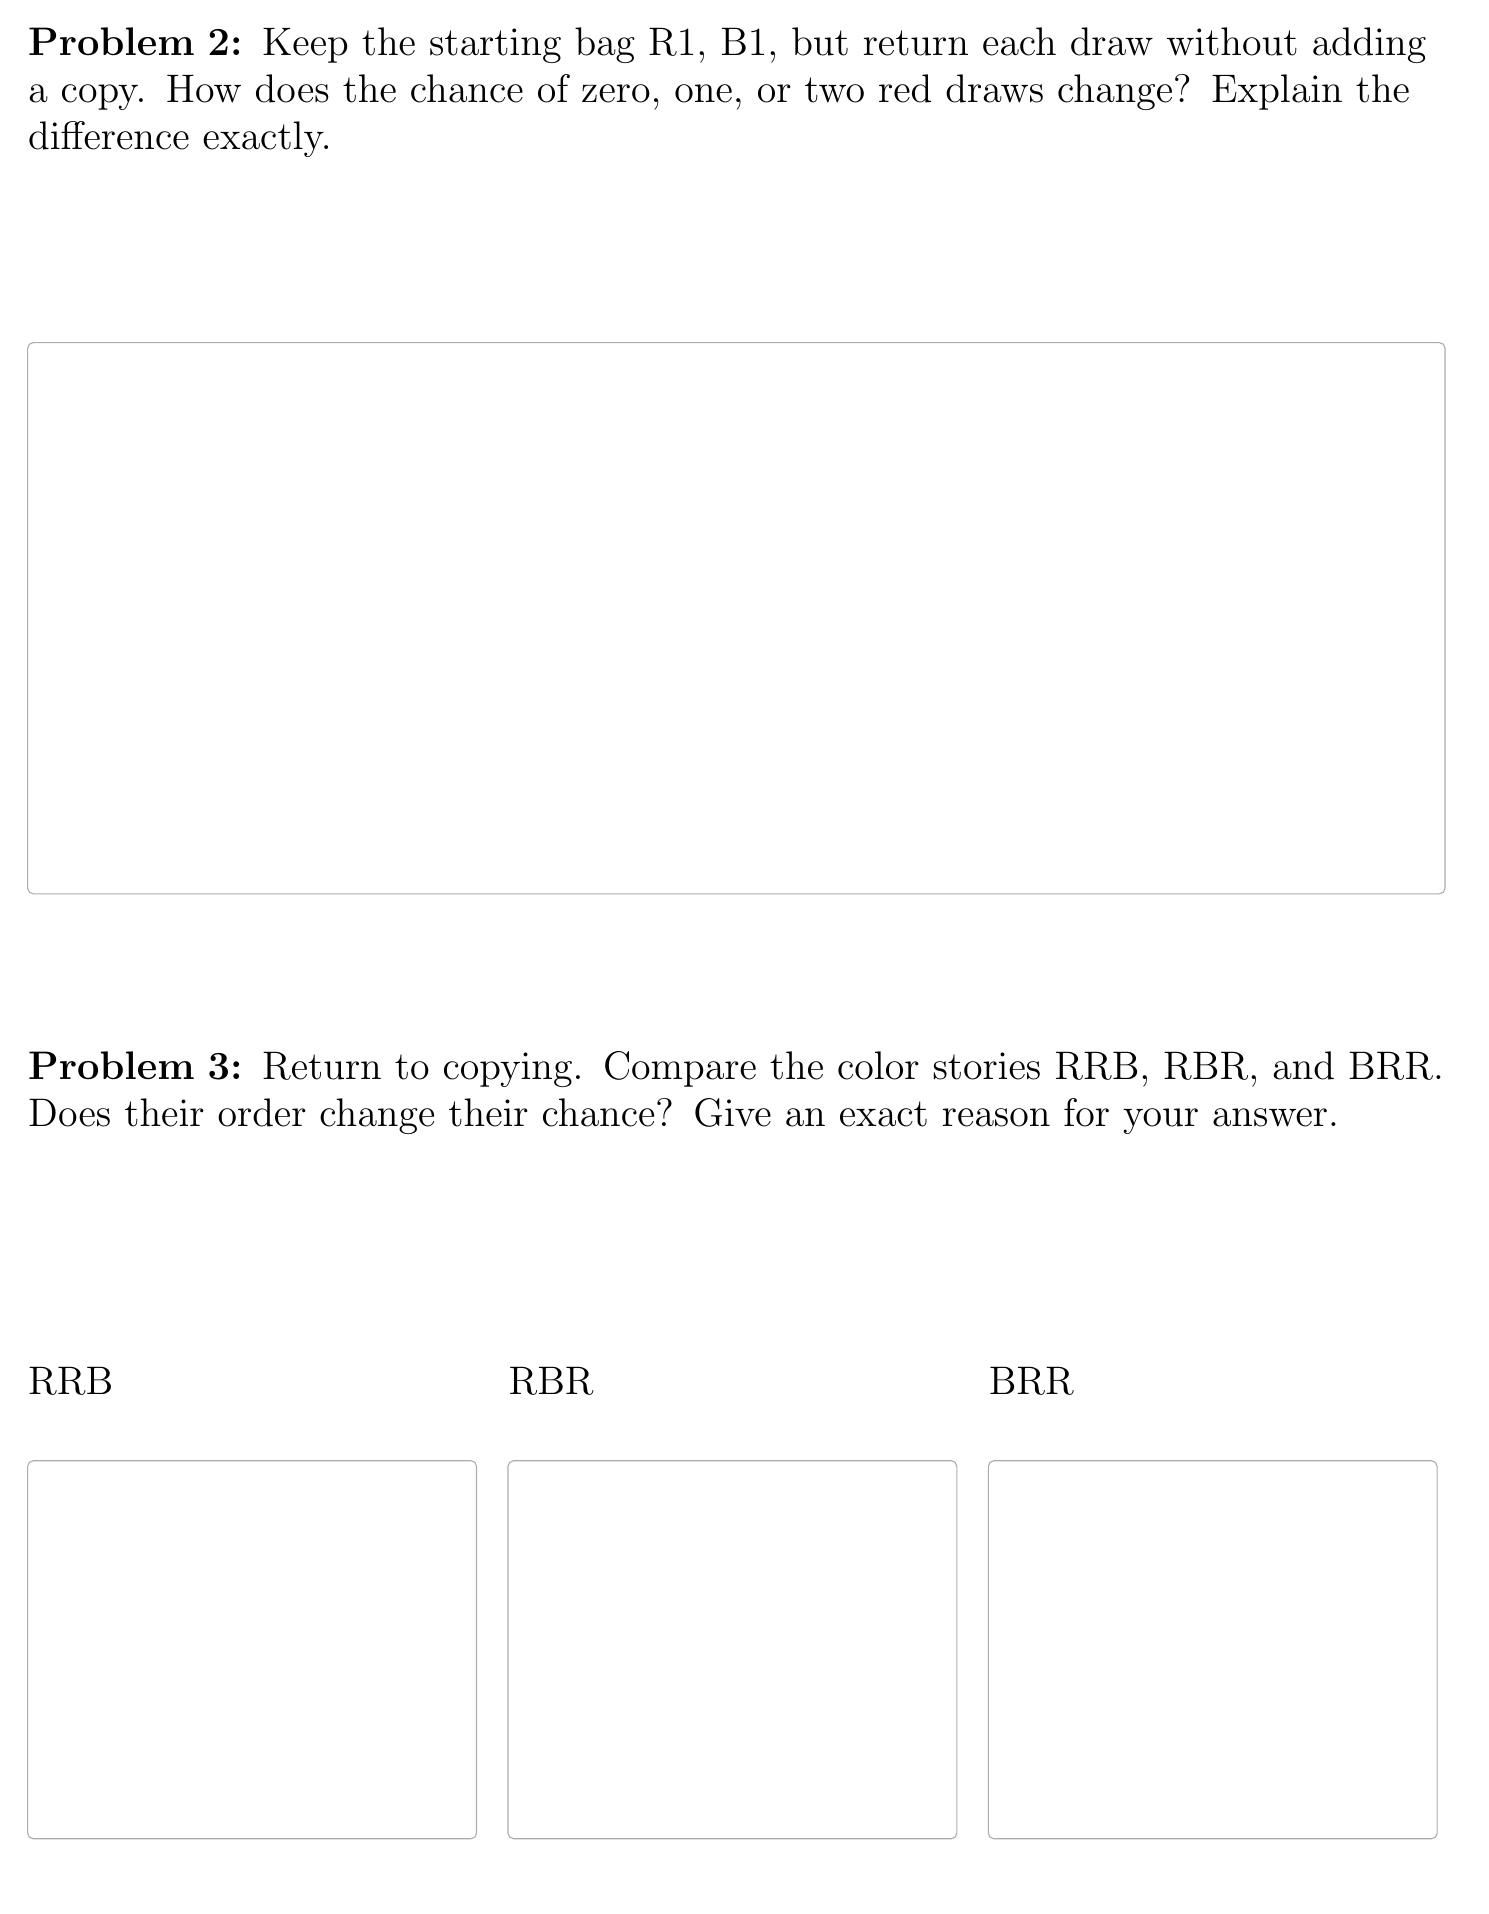
\begin{tikzpicture}[x=1cm,y=1cm]\path[use as bounding box] (0,0) rectangle (18.2,-23.6);
\node[anchor=north west,text width=18cm,inner sep=0pt,font=\fontsize{14}{17}\selectfont] at (0,0) {\textbf{Problem 2:} Keep the starting bag R1, B1, but return each draw without adding a copy. How does the chance of zero, one, or two red draws change? Explain the difference exactly.};
\draw[gray!65,rounded corners=2pt] (0,-4) rectangle (18,-11);
\node[anchor=north west,text width=18cm,inner sep=0pt,font=\fontsize{14}{17}\selectfont] at (0,-13) {\textbf{Problem 3:} Return to copying. Compare the color stories RRB, RBR, and BRR. Does their order change their chance? Give an exact reason for your answer.};
\node[anchor=north west,text width=5.7cm,inner sep=0pt,font=\fontsize{14}{17}\selectfont] at (0.0,-17) {RRB};
\draw[gray!65,rounded corners=2pt] (0.0,-18.2) rectangle (5.7,-23.0);
\node[anchor=north west,text width=5.7cm,inner sep=0pt,font=\fontsize{14}{17}\selectfont] at (6.1,-17) {RBR};
\draw[gray!65,rounded corners=2pt] (6.1,-18.2) rectangle (11.8,-23.0);
\node[anchor=north west,text width=5.7cm,inner sep=0pt,font=\fontsize{14}{17}\selectfont] at (12.2,-17) {BRR};
\draw[gray!65,rounded corners=2pt] (12.2,-18.2) rectangle (17.9,-23.0);
\end{tikzpicture}
\newpage
\noindent\begin{tikzpicture}[x=1cm,y=1cm]\path[use as bounding box] (0,0) rectangle (18.2,-23.6);
\node[anchor=north west,text width=18cm,inner sep=0pt,font=\fontsize{14}{17}\selectfont] at (0,0) {\textbf{Problem 4:} Three copying draws have 24 equally likely marked histories. How many give zero, one, two, or three red draws? Explain how you know your counts cover every possibility.};
\node[anchor=north west,text width=8cm,inner sep=0pt,font=\fontsize{14}{17}\selectfont] at (0.0,-4.0) {0 red draws};
\draw[gray!65,rounded corners=2pt] (0.0,-5.2) rectangle (8.0,-10.9);
\node[anchor=north west,text width=8cm,inner sep=0pt,font=\fontsize{14}{17}\selectfont] at (9.2,-4.0) {1 red draws};
\draw[gray!65,rounded corners=2pt] (9.2,-5.2) rectangle (17.2,-10.9);
\node[anchor=north west,text width=8cm,inner sep=0pt,font=\fontsize{14}{17}\selectfont] at (0.0,-12.2) {2 red draws};
\draw[gray!65,rounded corners=2pt] (0.0,-13.399999999999999) rectangle (8.0,-19.099999999999998);
\node[anchor=north west,text width=8cm,inner sep=0pt,font=\fontsize{14}{17}\selectfont] at (9.2,-12.2) {3 red draws};
\draw[gray!65,rounded corners=2pt] (9.2,-13.399999999999999) rectangle (17.2,-19.099999999999998);
\draw[gray!45] (0,-22) -- (18,-22);
\draw[gray!45] (0,-23) -- (18,-23);
\end{tikzpicture}
\newpage
\noindent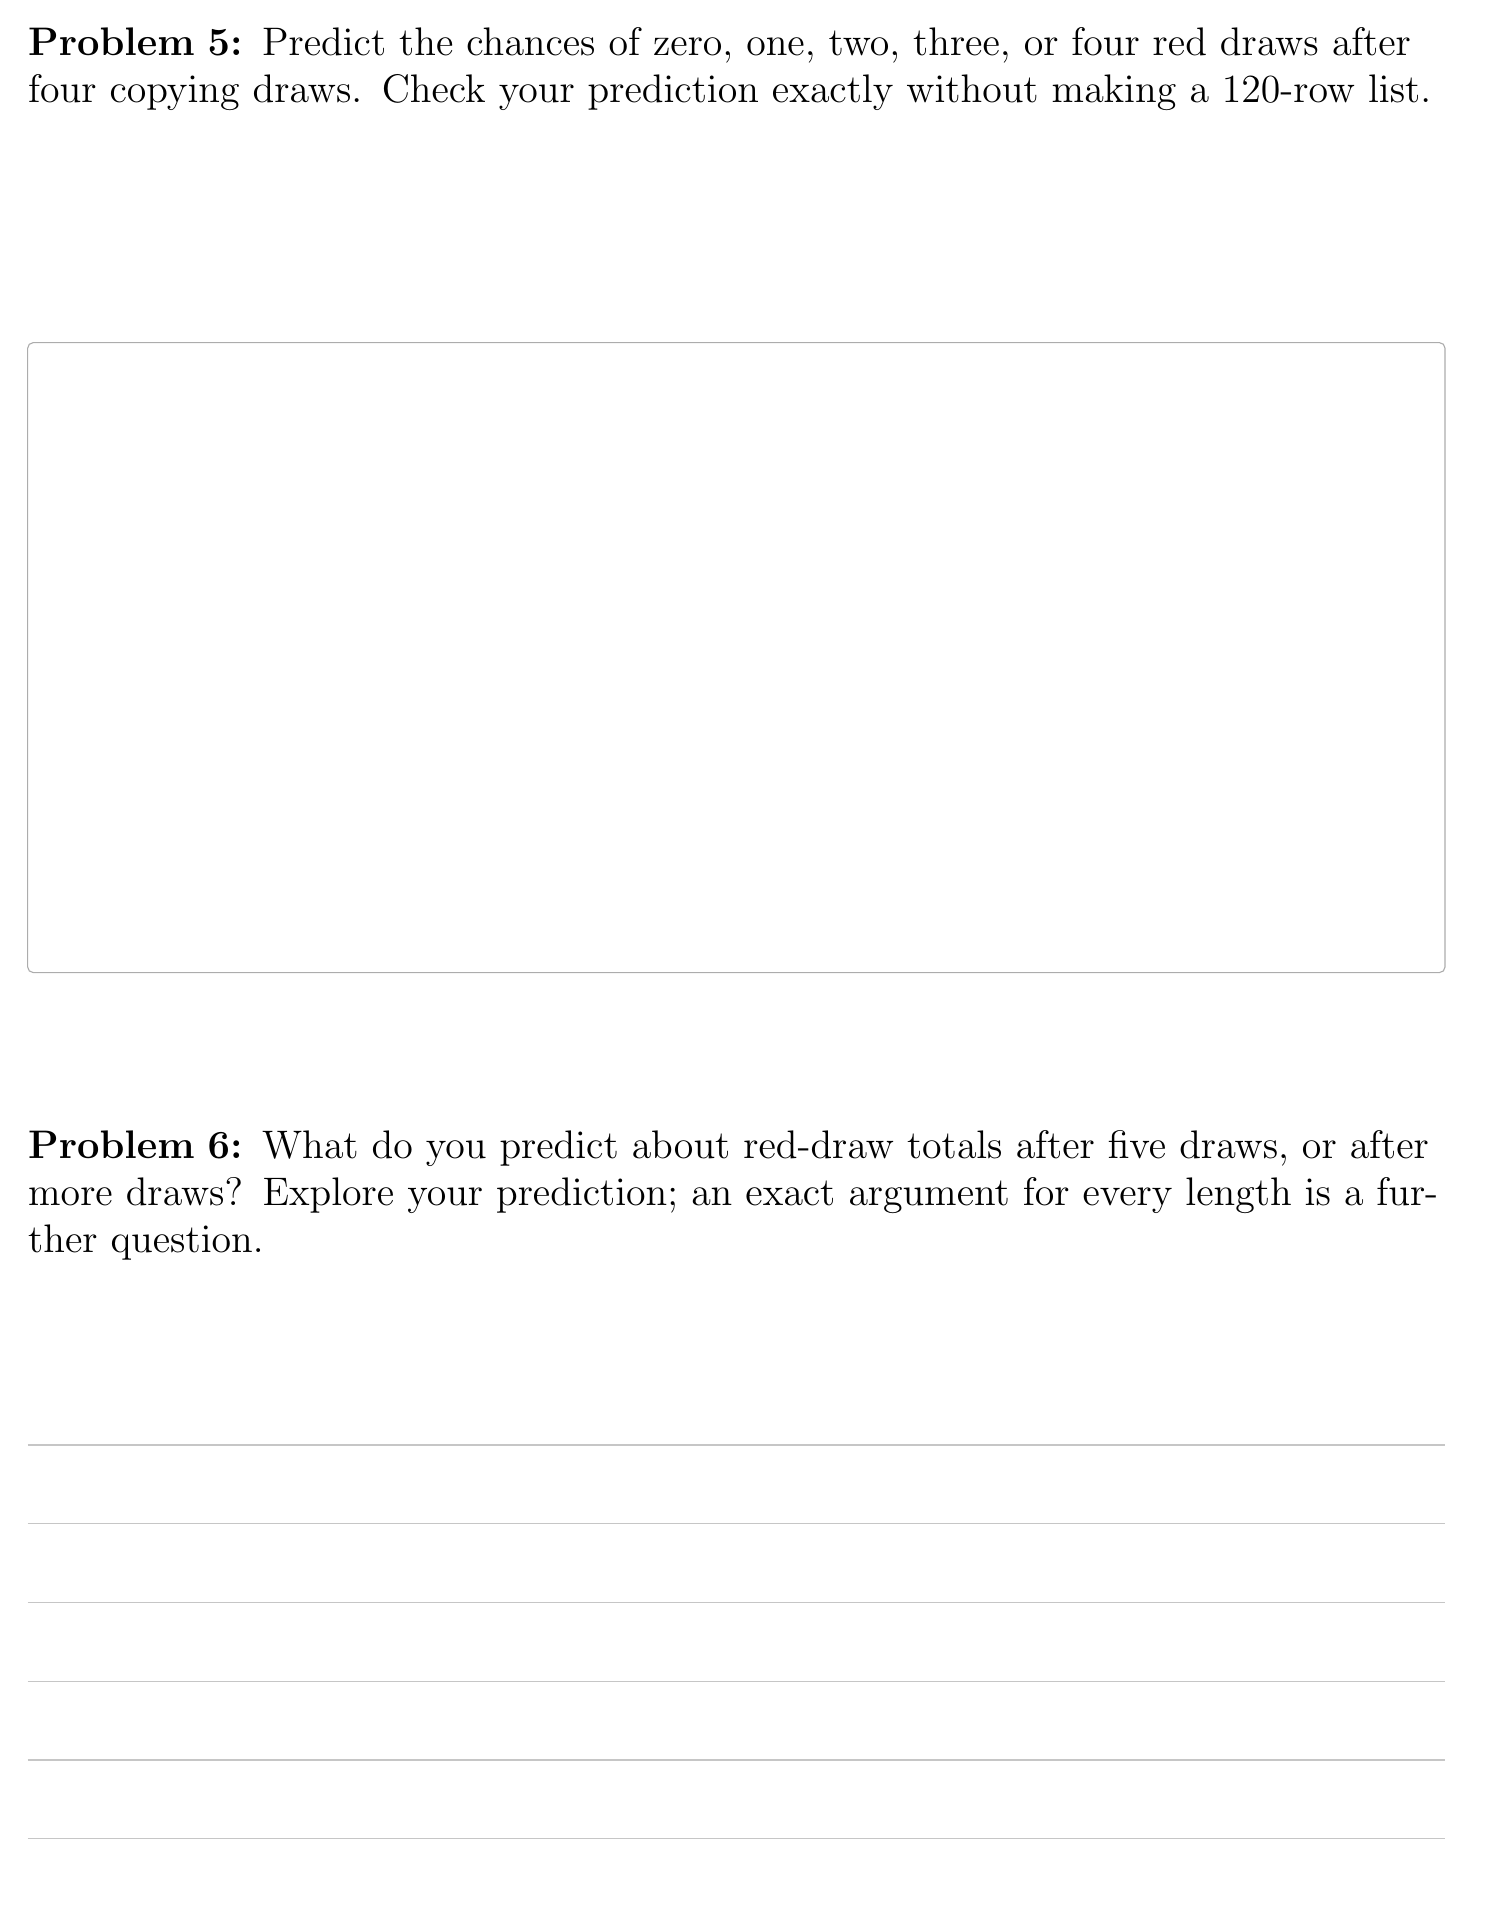
\begin{tikzpicture}[x=1cm,y=1cm]\path[use as bounding box] (0,0) rectangle (18.2,-23.6);
\node[anchor=north west,text width=18cm,inner sep=0pt,font=\fontsize{14}{17}\selectfont] at (0,0) {\textbf{Problem 5:} Predict the chances of zero, one, two, three, or four red draws after four copying draws. Check your prediction exactly without making a 120-row list.};
\draw[gray!65,rounded corners=2pt] (0,-4) rectangle (18,-12);
\node[anchor=north west,text width=18cm,inner sep=0pt,font=\fontsize{14}{17}\selectfont] at (0,-14) {\textbf{Problem 6:} What do you predict about red-draw totals after five draws, or after more draws? Explore your prediction; an exact argument for every length is a further question.};
\draw[gray!45] (0,-18) -- (18,-18);
\draw[gray!45] (0,-19) -- (18,-19);
\draw[gray!45] (0,-20) -- (18,-20);
\draw[gray!45] (0,-21) -- (18,-21);
\draw[gray!45] (0,-22) -- (18,-22);
\draw[gray!45] (0,-23) -- (18,-23);
\end{tikzpicture}
\end{document}
